\documentclass[11pt]{article}

% ── Fonts & Encoding ────────────────────────────────────────────
\usepackage[T1]{fontenc}
\usepackage{lmodern}
\usepackage{microtype}

% ── Math ────────────────────────────────────────────────────────
\usepackage{amsmath, amssymb, mathtools}

% ── Layout ──────────────────────────────────────────────────────
\usepackage[margin=1in]{geometry}
\usepackage{enumitem}
\usepackage{setspace}
\setstretch{1.15}
\setlength{\parindent}{0pt}
\setlength{\parskip}{0.6em}

% ── Colors & Boxes ──────────────────────────────────────────────
\usepackage[dvipsnames]{xcolor}
\usepackage{tcolorbox}
\tcbuselibrary{skins, breakable}

% ── TikZ (for diagram) ─────────────────────────────────────────
\usepackage{tikz}
\usetikzlibrary{arrows.meta, positioning, calc}

% ── Color palette ───────────────────────────────────────────────
\definecolor{accentblue}{HTML}{2563EB}
\definecolor{accentred}{HTML}{DC2626}
\definecolor{accentamber}{HTML}{D97706}
\definecolor{softgray}{HTML}{F3F4F6}
\definecolor{bordergray}{HTML}{D1D5DB}
\definecolor{darktext}{HTML}{1F2937}

% ── Custom tcolorbox styles ─────────────────────────────────────
\newtcolorbox{corequestion}{
  enhanced, breakable,
  colback  = accentblue!4,
  colframe = accentblue,
  coltitle = white,
  fonttitle = \bfseries\large,
  title = {Core Question},
  boxrule  = 0.8pt,
  arc      = 3pt,
  left     = 10pt, right = 10pt,
  top      = 8pt,  bottom = 8pt,
  shadow   = {1pt}{-1pt}{0pt}{black!15},
}

\newtcolorbox{issueblock}{
  enhanced, breakable,
  colback  = accentred!4,
  colframe = accentred!80!black,
  coltitle = white,
  fonttitle = \bfseries,
  title = {The Circular-Dependency Problem},
  boxrule  = 0.8pt,
  arc      = 3pt,
  left     = 10pt, right = 10pt,
  top      = 8pt,  bottom = 8pt,
  shadow   = {1pt}{-1pt}{0pt}{black!15},
}

\newtcolorbox{evidencebox}[1][]{
  enhanced, breakable,
  colback  = softgray,
  colframe = bordergray,
  fonttitle = \bfseries,
  boxrule  = 0.6pt,
  arc      = 3pt,
  left     = 10pt, right = 10pt,
  top      = 6pt,  bottom = 6pt,
  #1
}

% ── Hyperref (last) ────────────────────────────────────────────
\usepackage[colorlinks, linkcolor=accentblue, urlcolor=accentblue]{hyperref}

\begin{document}
\pagestyle{empty}
\color{darktext}

% ═══════════════════════════════════════════════════════════════
%  CORE QUESTION
% ═══════════════════════════════════════════════════════════════
\begin{corequestion}
The model requires a ground-truth-derived teleportation matrix~$E_i$ as input in order to simulate a given time frame.
How, then, can it \emph{forecast} a future time frame for which no ground truth exists?
\end{corequestion}

% ═══════════════════════════════════════════════════════════════
%  HOW THE MODEL WORKS
% ═══════════════════════════════════════════════════════════════
\textbf{\large How the Model Works}

\smallskip
We process one month of urban traffic data, divided into 15-minute frames.
For each frame~$i$ the model computes:
%
\[
  G_i \;=\; F\!\bigl(T,\; E_i\bigr),
\]
%
where the two inputs are:

\begin{itemize}[leftmargin=1.6em, itemsep=4pt]
  \item[\textcolor{accentblue}{\textbullet}]
    $T$ : the \textbf{transition matrix}, built from network topology and link features.\\
    \textit{This is independent of ground truth and is always available.}

  \item[\textcolor{accentred}{\textbullet}]
    $E_i$ : the \textbf{teleportation matrix}, derived \emph{directly from the ground-truth traffic distribution} for frame~$i$.\\
    \textit{This is the problematic input: it encodes the very answer the model is meant to produce.}
\end{itemize}

% ═══════════════════════════════════════════════════════════════
%  WHAT WE OBSERVE
% ═══════════════════════════════════════════════════════════════
\textbf{\large What We Observe}

\begin{evidencebox}[title={Observation 1 — Same-frame evaluation}]
When evaluated on the \emph{same} time frame that produced~$E_i$:
\[
  E_i \;\approx\; G_i
  \qquad\text{(relative error $\approx 0.02$).}
\]
This is unsurprising. The identity map $I(E_i) = E_i$ achieves the same result trivially.
The model ingests~$E_i$, applies stochastic processing, and returns an output nearly identical to the input, rendering the computation \textbf{redundant}.
\end{evidencebox}

\vspace{0.4em}

\begin{evidencebox}[title={Observation 2 — Cross-week prediction}]
To test genuine predictive power, we fed the teleportation matrix from a
\emph{Week~1} frame ($E_{i_1}$) into $F$ and measured how well it
predicted the corresponding \emph{Week~2} frame ($E_{i_2}$):
\[
  \frac{\lVert G_{i_2} - E_{i_2}\rVert}{\lVert E_{i_2}\rVert}
  \;\approx\; 0.4.
\]
Although this is a large improvement over earlier models (which had relative errors $\sim\!300$), \textbf{a 40\% relative error is still too high for reliable forecasting.}
\end{evidencebox}

% ═══════════════════════════════════════════════════════════════
%  THE ISSUE — VISUAL DIAGRAM
% ═══════════════════════════════════════════════════════════════
\begin{issueblock}

The architecture contains a fundamental circular dependency.
Consider the real use-case: \emph{simulate traffic in Salt Lake City for a specific
15-minute window in March~2026}.

\begin{center}
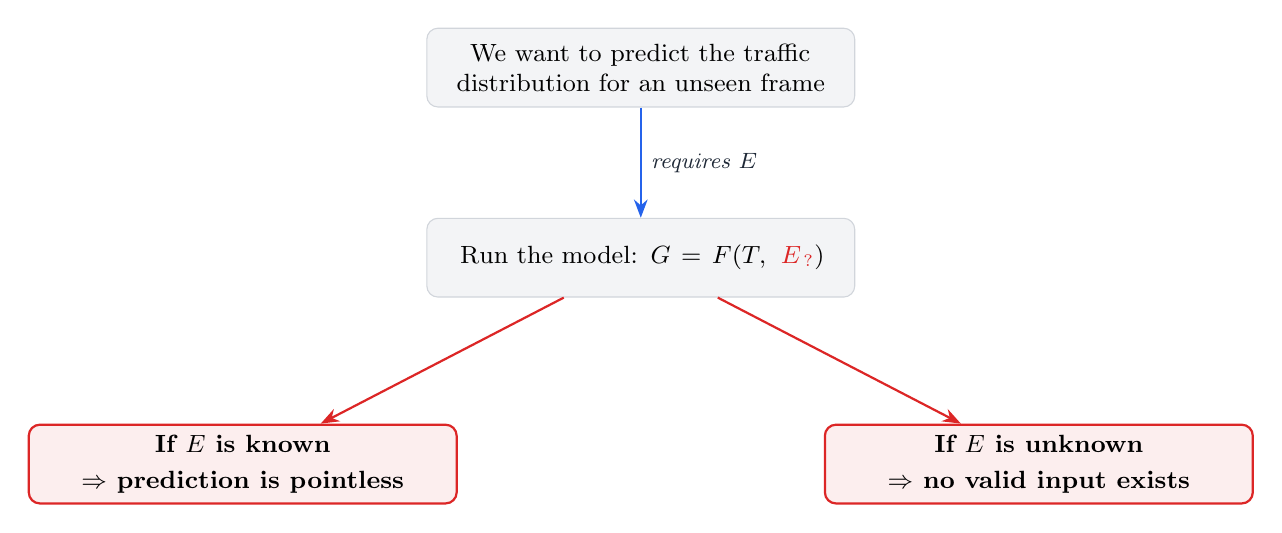
\begin{tikzpicture}[
    >=Stealth,
    node distance=2.8cm,
    box/.style={
      draw=bordergray, rounded corners=4pt,
      fill=softgray, minimum height=1cm,
      text width=5.2cm, align=center, font=\small
    },
    deadend/.style={
      draw=accentred, thick, rounded corners=4pt,
      fill=accentred!8, minimum height=1cm,
      text width=5.2cm, align=center, font=\small\bfseries
    }
  ]

  \node[box] (goal)
    {We want to predict the traffic distribution for an unseen frame};

  \node[box, below=1.4cm of goal] (model)
    {Run the model: $G = F(T, \;{\color{accentred}E_{\,?}})$};

  \node[deadend, below left=1.6cm and -0.4cm of model] (known)
    {If $E$ is known\\[2pt] $\Rightarrow$ prediction is pointless};

  \node[deadend, below right=1.6cm and -0.4cm of model] (unknown)
    {If $E$ is unknown\\[2pt] $\Rightarrow$ no valid input exists};

  \draw[->, thick, accentblue] (goal) -- (model)
    node[midway, right, font=\footnotesize\itshape, text=darktext] {requires $E$};
  \draw[->, thick, accentred]  (model) -- (known);
  \draw[->, thick, accentred]  (model) -- (unknown);

\end{tikzpicture}
\end{center}

In both branches, the model fails to serve as a practical simulator:
\begin{enumerate}[leftmargin=1.6em, itemsep=3pt, label=\textcolor{accentred}{\arabic*.}]
  \item \textbf{Ground truth is available.}
        Feeding it in is redundant, we already have what we want.
  \item \textbf{Ground truth is unavailable} (the realistic case).
        There is no valid teleportation matrix to supply, so the model \emph{cannot run}.
\end{enumerate}

\end{issueblock}

\vspace{0.6em}

\textbf{\large The Open Question}

\smallskip
What should be used as the teleportation input~$E$ so that the model becomes a
viable, practical simulator for \emph{unknown} future time frames?

\end{document}